\subsection{Data import and preprocessing}

\noindent The color images that make up the dataset (called \textit{observations}), once imported into the work environment, can be represented as tensors, each $96\times96\times3$ in size ($96$ pixels high, as many wide, and $3$ RGB color channels). They are originally grouped in folders that are labeled with the class id to which they belong, corresponding to the action of the car in the racing video game: a random sample is shown in Fig. \ref{fig:sample}.

\noindent \\In total, 9,118 samples are available, of which 6,369 belong to the training set and the remaining 2,749 to the validation set. However, the classes are not balanced in terms of the number of elements, and nor does this imbalance occur in the same way in the two subsets (see Fig. \ref{fig:train_set} and \ref{fig:test_set}).
\\Since it would not be fair to modify the way the subsets are split, this suggests that accuracy problems may arise in the solution. In fact, in general, the division between the training and validation sets should occur randomly, and consequently, they should be distributed in the same way even if class-imbalanced.
\\Furthermore, another question arises: how well does the training set represent the "correct" behavioral model of the player in the Car Racing environment? Based on the answer to this question, we will obtain a model capable of navigating the race track or one that will crash the car at the first turn.
\begin{figure}[htbp]
    \centering
    \subfloat[Training set.]{
        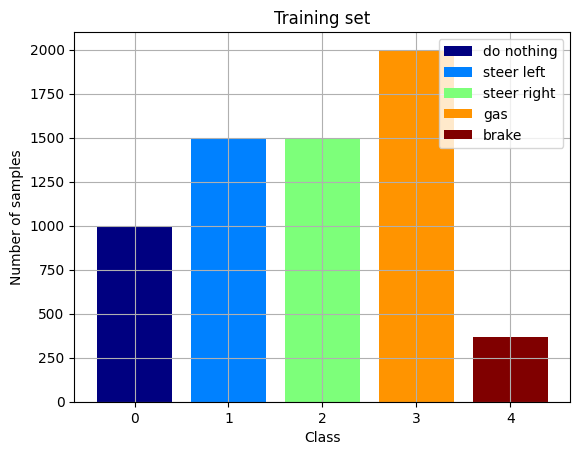
\includegraphics[width=0.4\textwidth]{figures/images/train_set.png}
        \label{fig:train_set}
    }
    \subfloat[Validation set.]{
        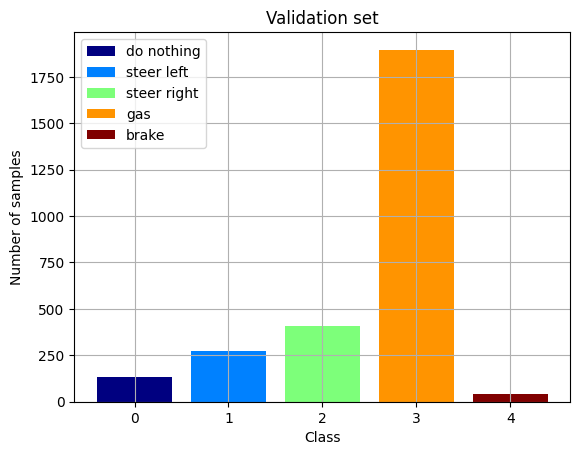
\includegraphics[width=0.4\textwidth]{figures/images/test_set.png}
        \label{fig:test_set}
    }
    \caption{Composition of the dataset.}
\end{figure}

\noindent \\Another aspect to consider is the information contained in a single observation. In fact, it is common practice to preprocess images before feeding them into a classification model (both instances belonging to the dataset and not), mainly to reduce computational load and to improve training performance.
\\For this particular problem, the following manipulations are applied:

\begin{enumerate}
    \item the texture of the grass is made uniform;
    \item the saturation is enhanced;
    \item the colors are converted to grayscale;
    \item the reward counter in the lower left corner is concealed;
    \item the elements of the tensor are normalized to 1.
\end{enumerate}

\noindent This way, we expect the model to converge more easily to an acceptable solution and to have fewer issues in generalizing what it will learn from the data. \\In Fig. \ref{fig:sample_preprocessed} the preprocessing of the previous random sample is carried out as an example.
\begin{figure}[htbp]
    \centering
    \subfloat[A random sample of the dataset.]{
        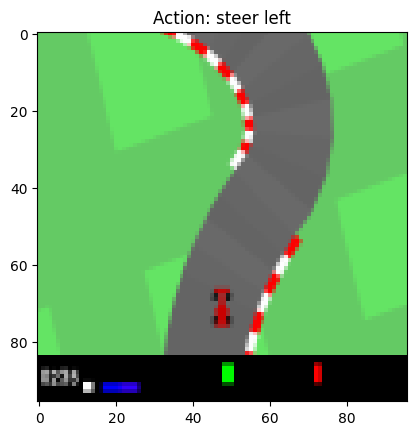
\includegraphics[width=0.35\textwidth]{figures/images/sample.png}
        \label{fig:sample}
    }
    \subfloat[The same sample after preprocessing.]{
        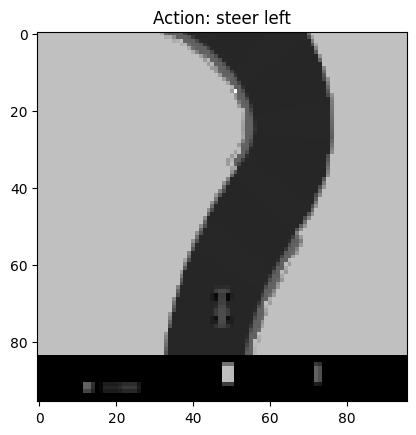
\includegraphics[width=0.35\textwidth]{figures/images/sample_preprocessed.png}
        \label{fig:sample_preprocessed}
    }
    \caption{Effect of preprocessing on the observations.}
\end{figure}